%% Copyright (C) 2009 by Tobias Elze
%% Journal of Vision LaTeX template version 1.0
%% This document may be used freely for your own submissions.

\documentclass{jov}
\usepackage[mediumspace,mediumqspace,Grey,squaren]{SIunits}

 \usepackage{graphicx}
 \usepackage{mathtools}
 \usepackage{amsmath}
 \usepackage{setspace}
 \usepackage{tikz}
 \usepackage{url}


\newenvironment{enoomerate}{
\begin{enumerate}
  \setlength{\itemsep}{1pt}
  \setlength{\parskip}{0pt}
  \setlength{\parsep}{0pt}}{\end{enumerate}
}

\newenvironment{itemise}{
\begin{itemize}
  \setlength{\itemsep}{1pt}
  \setlength{\parskip}{0pt}
  \setlength{\parsep}{0pt}}{\end{itemize}
}



\newcommand{\up}[1]{\ensuremath{^{\textrm{#1}}}}
\newcommand{\down}[1]{\ensuremath{_{\textrm{#1}}}}

\newcommand{\Xangstrom}{\r{a}ngstr\"{o}m}


\newcommand{\Xth}{\up{\tiny{th}}}
\newcommand{\st}{\up{\small{st}}}
\newcommand{\nd}{\up{\small{nd}}}
\newcommand{\rd}{\up{\small{rd}}}

\newcommand{\Xeta}{\textit{et al }}
\newcommand{\Xiv}{\textit{in vivo }}
\newcommand{\Xxv}{\textit{ex vivo }}
\newcommand{\Xis}{\textit{in silico }}

\newcommand{\etal}{\textit{et al }}
\newcommand{\invivo}{\textit{in vivo }}
\newcommand{\exvivo}{\textit{ex vivo }}
\newcommand{\insilico}{\textit{in silico }}
\newcommand{\invitro}{\textit{in vitro }}

\newcommand{\um}{\micro m}

\newcommand{\xa}{\textit{a) }}
\newcommand{\xb}{\textit{b) }}
\newcommand{\xc}{\textit{c) }}
\newcommand{\xd}{\textit{d) }}
\newcommand{\xe}{\textit{e) }}

%DOCUMENT-SPECIFIC COMMANDS

 \newcommand{\pcatwo}{PCA\up{2} }




%\begin{figure}[htp]
%\centering
%\includegraphics[scale=0.5]{img/bubbles.png}
%\caption{Bubbles in the right atrium (RA) and vena cava (VC) of a guinea pig after decompression from 0.4MPa. From \cite{daniels1980detection}. Approximate scale: the area shown   in the image measures several mm across.}
%\label{bubbles}
%\end{figure}

%width = /textwidth
\usepackage{subfig}

\begin{document}

\title{This is the title of the article}
\abstract{This document is an inofficial \LaTeX{} template to be used
to create a suitably formatted submission for the Journal of Vision. It
considers the changed layout requirements as of 2010. The complete
instructions for manuscript preparation are available at
\href{http://www.journalofvision.org/site/misc/ifora.xhtml}
{http://www.journalofvision.org/site/misc/ifora.xhtml}.
This is the text of the abstract. This version of the template is dated
\today. The template makes your \LaTeX{} manuscript look similar to 
Journal of Vision articles. However, in contrast to the two-column JOV
articles, manuscripts are in single colum mode.}

\author{Smith}{Jane Q.}
 {Schepens Eye Research Institute}
 {and Harvard Medical School, Boston, MA, USA}
 {http://}{jqs@schepens.harvard.edu}
\author{Elze}{Tobias}
 {Research Group Complex Structures in Biology and Cognition}
 {Max Planck Institute for Mathematics in the Sciences, Leipzig, Germany}
 {http://www.mis.mpg.de/complex/members/tobias-elze.html}
 {Tobias.Elze@mis.mpg.de}

\keywords{reverse correlation, triggered correlation, primate, recursive 
least squares, linear-nonlinear model, system identification}

\maketitle

\section{Introduction}


Fire is a complex and dynamic phenomenon. Characterised by rapidly shifting patterns of both first- and second-order motion, it evokes rich visual percepts as well as aesthetic responses. We report an investigation of the visual features useful for discrimination between similar fires, the neurocognitive architecture responsible for comparing them, and the specificity of the neural representations involved.


From an evolutionary point of view, mastery of fire was key to human development. Being able to control fire allowed early humans to cook food, defend themselves from predators and survive in cold, challenging environments. Fire was the first of a long line of technologies which release stored energy from fuel and turn it to human purposes; the earliest archaeological evidence of fire use dates back 1.8 million years (REF), with frequent use found from (FILL) million years onwards (REF). Even before this, hominids regularly encountered flame in the form of bushfires, although these were perceived as a threat, not a controllable, exploitable entity.

The evolving human visual system has therefore been exposed to a large amount of flamelike stimuli in the last 1.8 million years. These stimuli have often appeared in dangerous or life-threatening contexts, either posing a threat or aiding survival. In sufficiently extreme situations, such as extreme cold or heavy predation, those early humans who could successfully control fire had an increased chance of survival.

It is therefore natural to enquire whether the human visual system has become adapted in any way to the perception of flamelike stimuli. Does the visual system employ any specific representations or specialised models when attending to fire, does it use the same general-purpose systems employed when observing a novel moving stimulus?

This question recalls the ongoing debate concerning the specialisation of face perception. We find increased activation of the fusiform face area and inferior temporal sulcus while viewing faces; this can be explained either by innate specialisation or learned proficiency. In the same way, observation of fire may recruit neurons and systems which respond preferentially to, and perform better on, flame stimuli. On the other hand, observing fire may stimulate the same neural populations as observing other moving stimuli.

This report aims to answer two questions. Firstly, what types of visual information are important when observing flames; which details are represented, and which thrown away? This choice defines the upstream visual subsystems (for example, that of motion detection, edge detection or shape detection) which are activated by fire stimuli. Secondly, are any of these systems specific to fire? We do not address the question of whether any specificity is learned or innate.

We begin with a survey of the ecological context in which fire is observed and processed. We then describe several yes/no and 2AFC tasks designed to activate the visual subsystems which process fire and measure task performance under removal of different types of visual information from the stimulus.

\section{Fire in the natural environment}

Here we swiftly review the basic characteristics of fire and the contexts in which early humans interacted with it. It is essential to consider the motivations and tasks which lead the visual system to process and represent fire.

We can define the set of dynamic visual stimuli termed "fire" as the light fields emitted from combusting objects. In terms of luminance, they display rapid variation from gentle glows to dazzling flares, which covers virtually the whole photopic range of the visual system; one can imagine that scotopic vision is not employed except for very dim, distant fires. In terms of size, they may subtend any angle from the whole visual field (for a large, close fire) to a point (for a small, distant fire).

In terms of spatial frequency, fire is characterised by 

FFT stuff here

It is important to consider the context in which flames were observed by early humans. We can imagine two main situations: a) avoiding large natural wildfires, and b) controlling small artificial hearth fires for cooking and defence. Good performance at both tasks is essential for survival, but we are not as interested in visual development supporting task performance in situation a), as it is not specific to humans; all large land animals in an environment at risk of wildfires must possess this skill. We consider only the anthrospecific task of controlling small artificial fires.

Fire is employed in many situations, from defensive to culinary to ritualistic. In order to avoid being overly selective, we do not consider a particular task, but the general context in which they can all be placed: the extraction of useful information (or affordance) from visual stimuli. In order to properly control a fire, the observer must estimate properties such as the temperature of various parts, whether the fire is growing or shrinking, whether it is likely to spark or flare up, and in which direction it will spread. Knowing these details accurately is especially important in the early stages of firelighting, when the flame is small and at risk of extinguishing.

We therefore restrict this work to the study of small, artificial fires which do not pose an imminent threat to survival. 

\section{How is fire represented?}

Any visual stimulus is coded using a large set of varyingly structured representations, varying in their cortical location and information content.

We investigated flame perception psychophysically using a delayed match-to-sample task involving short video clips of a hearth fire. In each trial, subjects viewed a sample clip followed by two slightly longer candidate clips, one of which contained the sample. The candidates were made longer due because the increased recognisability of start and end frames allowed matching to be done without attending to the rest of the sample. Subjects were asked to indicate in which candidate the sample was present, and their performance measured.

The cognitive process being tested was thus one of perception and comparison between a sample and two candidates. Although this task is not a perfect analogue of the ecological contexts in which fire is perceived (which involve evaluation of one fire, rather than comparison of two), it allows us to characterise the neural representations involved, as they play a key part in the discrimination process.

We can model this task in three stages: perception, representation, and output (see Fig. REF). It is tempting to dissociate the representation stage into perception (encoding of the stimuli) and comparison (a separate process acting to compare the encodings), as would occur in the storage and comparison of video clips on a computer. Neurally, however, we cannot assume that these processes are separate; representation and comparison may share the same neural apparatus.

We used this matching paradigm in a series of experiments to characterise the comparison process and thus the representations involved. We first showed that matching is not done by a process analogue to convolution. We then showed that different types of visual information (colour, spatial form, and temporal order) play very different parts in constructing representations of fire.

\section{Post-comparison or convolution?}

The process of representation is straightforward to imagine: we can see it as a function mapping visual inputs to neural states. It is useful to divide the overall neural state into separate representations (as in dorsal/ventral visual stream theory). Representation involves the eyes, early visual system and visual cortex. The process of comparison is more difficult: overall, it can be seen as a function mapping neural states to a binary response (the yes/no signal recorded by the experimental setup). Comparison involves task-oriented function and finally motor control.

One characteristic of the comparison process is easy to determine psychophysically: whether or not it is analogous to convolution, a process via which one small sample pattern is "slid along" or "moved over" a large candidate pattern (usually an image, signal or matrix). As it goes, the small pattern is compared locally to the large pattern. Convolution is characterised by independence from candidate pattern size: as the comparison is local, any matching areas of the candidate pattern will be detected even if it is very large.

We looked for this size-independence property in the fire comparison task by varying the candidate clip length in the matching paradigm. In Experiment 1 (see Fig. REF), sample length was varied (between blocks) between 10 and 50 frames (0.2 and 1 seconds). The ratio of sample length to candidate length was varied (within blocks) between 1.2 and 2 (candidates up to twice as long as targets).

Our predictions were as follows. If comparison was being done by a process analogous to convolution, samples would match up equally well against short candidates and long candidates. The matching region would be detected by local comparison. Therefore, accuracy would not depend on candidate length. On the other hand, if the comparison process were more global, longer candidates would be matched less efficiently due to constraints on the comparison process.

As shown in Fig. REF, candidate ratio has a highly significant negative effect on accuracy. Apart from comparison dynamics (whether or not comparison is convolution-esque), there is another consideration which could produce this effect: stimulus confusability.

Assuming a convolution-esque comparison process

Because the comparison process is not perfect, it is possible for areas in the candidate to be erroneously matched to the target (confused). Because fire is a repetitive, self-similar stimulus, the longer the candidate, the higher the likelihood that confusable areas will appear in the target. This, as opposed to non-convolution-like behaviour, could cause the negative effect of candidate ratio on accuracy.

To rule this out, we investigated the effect of varying sample length on performance (Experiment 2). If the stimulus was highly confusable, longer samples would stand a higher chance of being falsely matched with candidates, which would decrease accuracy. If not, longer samples would provide more useful information, increasing accuracy.

Experiment 2 followed the same match-candidates-to-sample paradigm. This time, sample length was varied (within blocks) between 1 and 12 frames (0.02 and 0.24 seconds), while target length was varied (across blocks) between 15 and 20 frames (0.3 and 0.4 seconds).

As shown in Fig, REF, sample length had a highly significant positive effect on accuracy. Longer samples were easier to match. If longer samples were more confusable due to self-similarity, a negative effect of sample length on accuracy would have been expected.

(image-based work)


In a delayed-match-to-sample task, sample length has a positive effect on subject accuracy, whereas candidate length has a negative effect. If the latter effect were due to  higher confusability between samples and longer candidates, we would not have seen the former effect. We thus conclude that the neural comparison process is not analogous to convolution, and that there are constraints in place which make it less effective on longer candidates.

These constraints may stem from the nature of the representations involved: global encodings may hold the same amount of information about the stimulus, independent of its length. This would lead to more information loss for longer candidate stimuli, and thus a loss of accuracy.

Constraints may also be temporal: even given perfect representations, the process which compares them may be time-limited for efficiency. Comparing perceived objects to representations is a core, often time-critical visual task. The comparison process may therefore permit more information loss, and lower accuracy, when acting on longer representations of larger clips.

(We could test this by not giving much time to perform the comparison). 

  \begin{figure}[!ht]
\centering
    \subfloat[A delayed match-to-sample paradigm was re-used several times in this study. Subjects selected which of two candidate clips contained a slightly shorter sample clip. Accuracy ranged from 50\% to 100\%.\label{subfig-1:dummy}]{%
      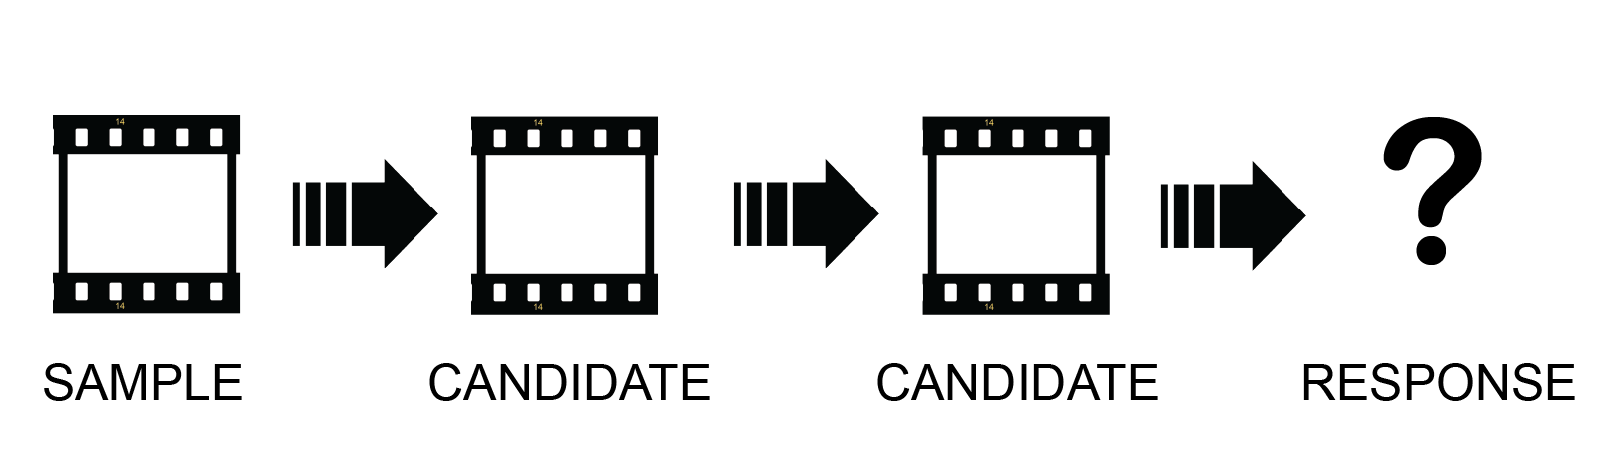
\includegraphics[width=0.9\textwidth]{img/protocol1.png}
    }
 

    \subfloat[\textbf{Experiment 1.} Increasing candidate length lowered accuracy, showing that the sample-candidate comparison process depends on candidate length.\label{subfig-2:dummy}]{%
      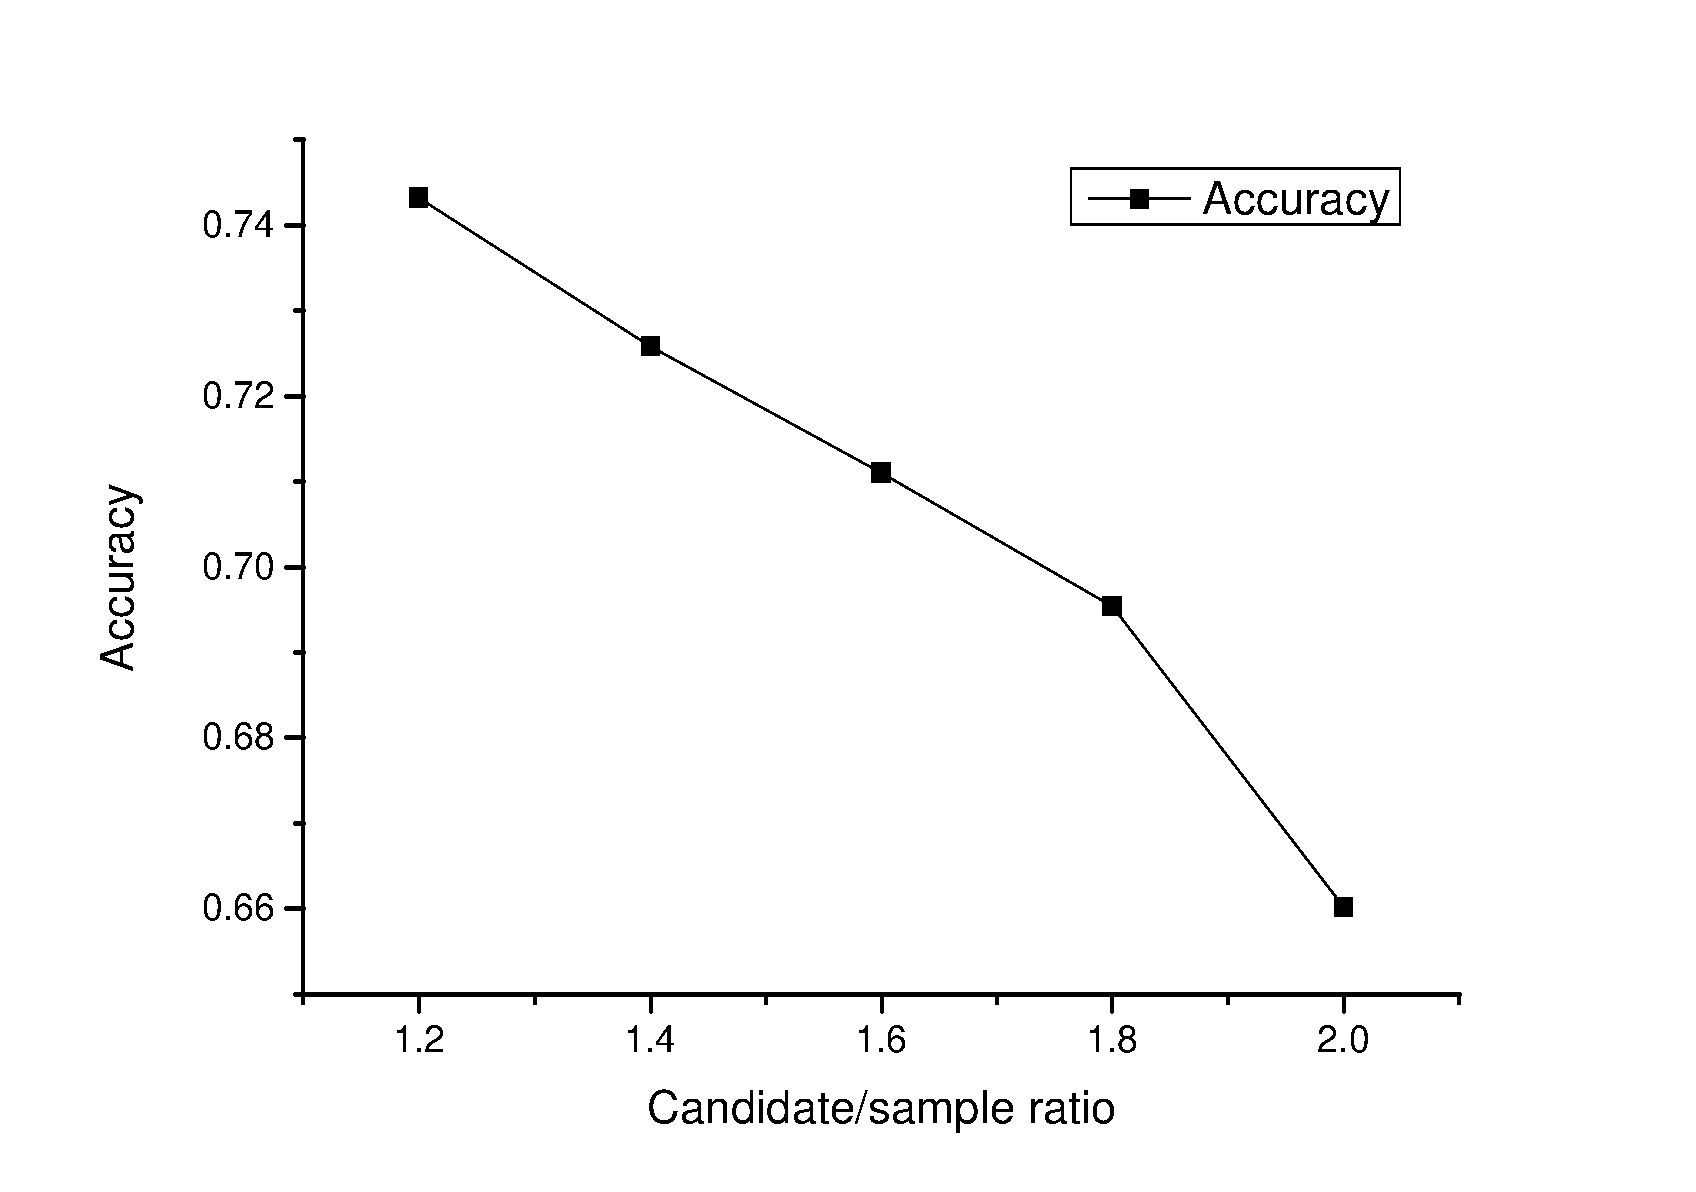
\includegraphics[width=0.45\textwidth]{img/accuracyvsratio.pdf}
    }
\hspace{0.3cm}
\subfloat[\textbf{Experiment 2.} Increasing sample length raised accuracy, showing that longer samples aid recognition.\label{subfig-2:dummy}]{%
      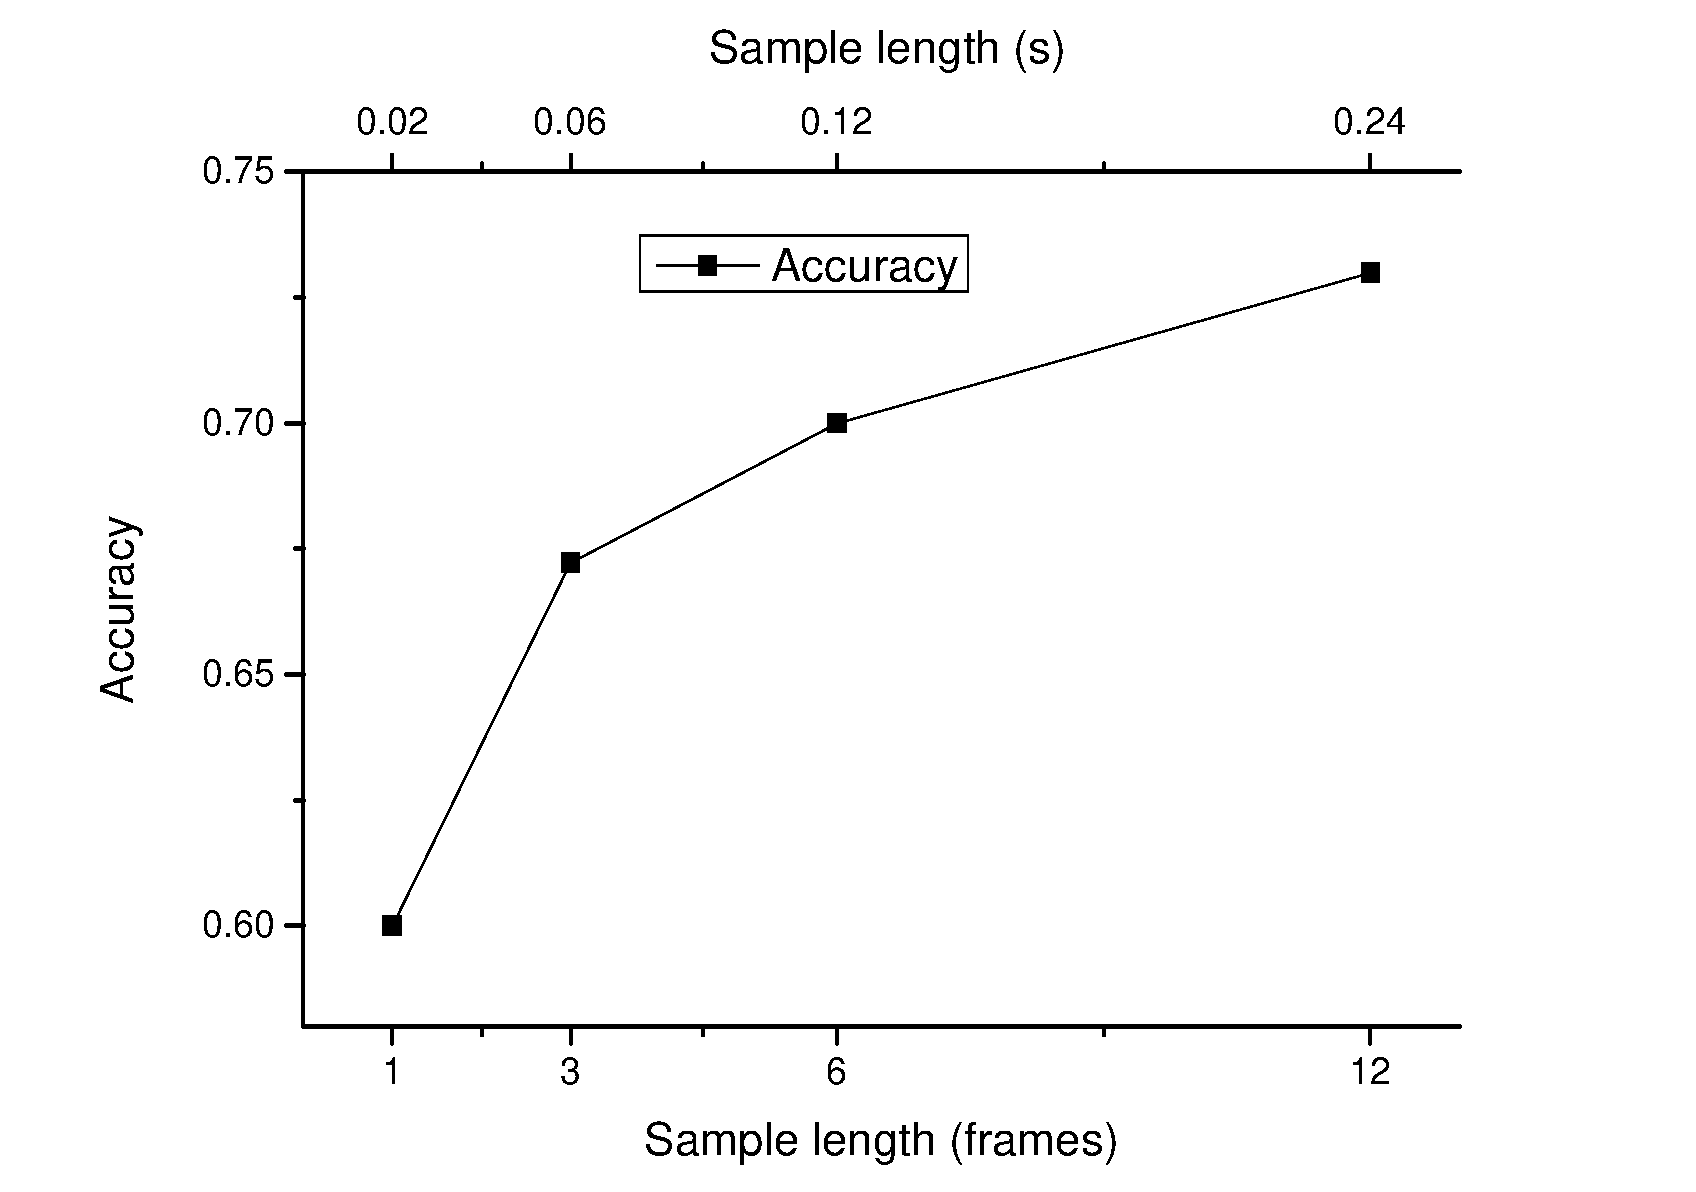
\includegraphics[width=0.45\textwidth]{img/accuracyvssamplelength.pdf}
    }
    \caption{In a delayed match-to-sample task, subjects were asked to select which of two candidate clips contained a target clip. Accuracy decreased with candidate length, showing that the comparison process is not analogous to convolution. Accuracy increased with sample length; the previous effect is therefore not due to higher clips being more confusable.}
    \label{fig:dummy}
  \end{figure}

\section{What do these representations describe?}

Representations are built from a range of visual features such as object boundaries, colour, motion, texture and contour. We investigated the relative importance of these ingredients in the representation and comparison of fire. The same delayed-match-to-sample paradigm was employed, with an important difference: the sample was modified to remove some of its information. 

Consider showing a monochrome sample clip, with missing colour information, followed by two full-colour candidate clips. The representation set evoked by the sample is therefore lacking in colour information from the sample (in specialised representations, colour may be filled in according to an internal model, but will not correspond to the sample's actual colour).

The candidate clips, on the other hand, are represented with their real colour. The process which compares candidates to samples must therefore match a detail-lacking representation to a detail-rich one. If the missing details are an important part of the representations, matching accuracy will suffer; however, the absence of unimportant details will not impact accuracy.

In Experiment 3 we removed three types of visual information from the samples: colour (by using monochrome clips), spatial arrangement (by rotating the samples through 180 degrees) and temporal arrangement (by playing the samples backwards). We measured the relative effect on accuracy of removing each detail.

Sample manipulation was varied between blocks. Each alteration was presented across 4 separate blocks, along with 4 control blocks whose samples were unmodified. The order of the set of 16 blocks was randomised.

The manipulation with the greatest effect on accuracy was temporal inversion...

(write up)


We thus conclude that, in the set of representations accessible to the comparison process, colour is of much less importance than spatial and temporal form. The perception and recall of flame is therefore closely linked with the spatial arrangement, and the motion, of perceived image features.


  \begin{figure}[!ht]
\centering
    \subfloat[To alter their natural colour, clips were processed by expression in HSV colour space and rotation through 180\degree in the hue plane. Clips were also inverted. \label{subfig-2:dummy}]{%
      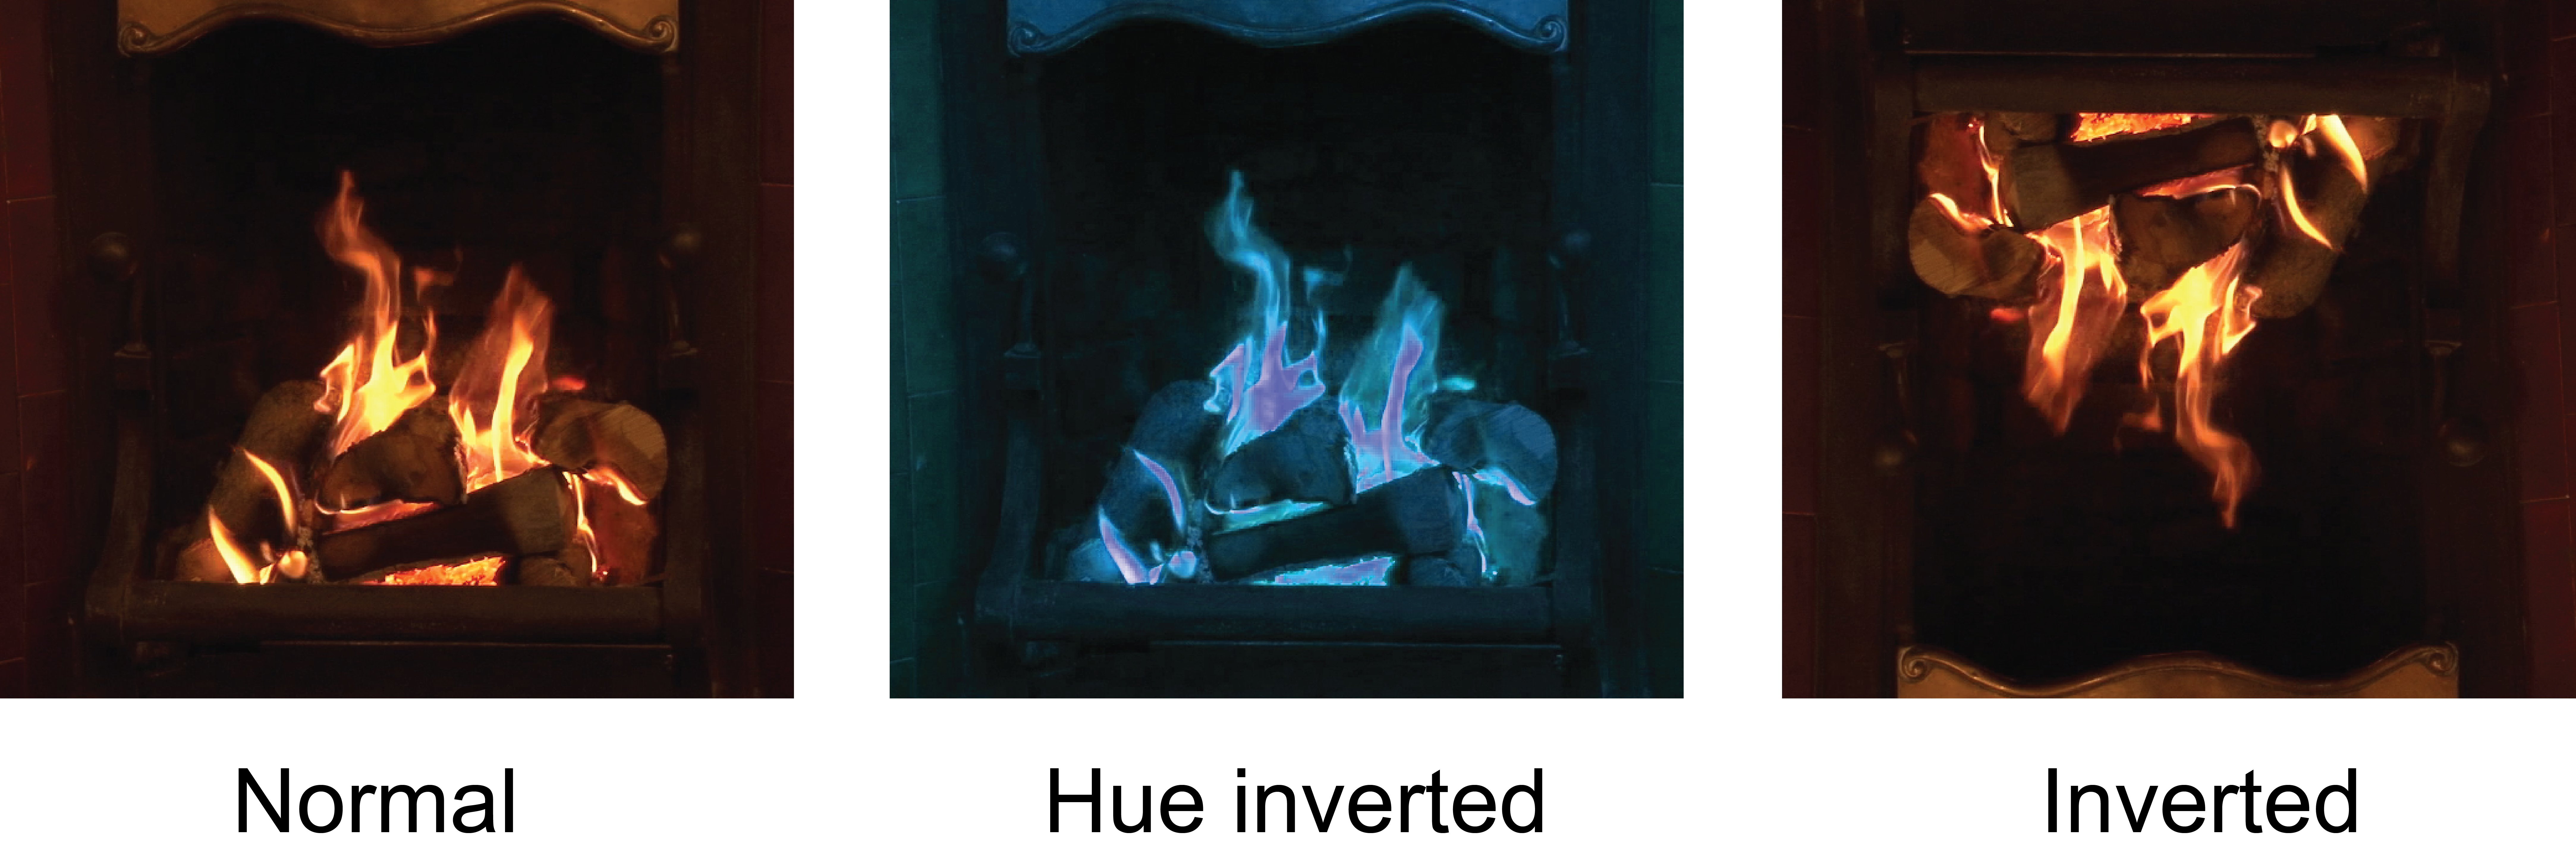
\includegraphics[width=\textwidth]{img/manipulations.png}
    }
\hspace{0.3cm}

\subfloat[The delayed match-to-sample paradigm was reapplied, with alterations (conversion to monochrome, reversed playback, and inverted playback) made to the sample only. Encodings of the sample, with partial information, thus had to be matched to unaltered candidates. Error bars show 95\% confidence intervals.\label{subfig-2:dummy}]{%
      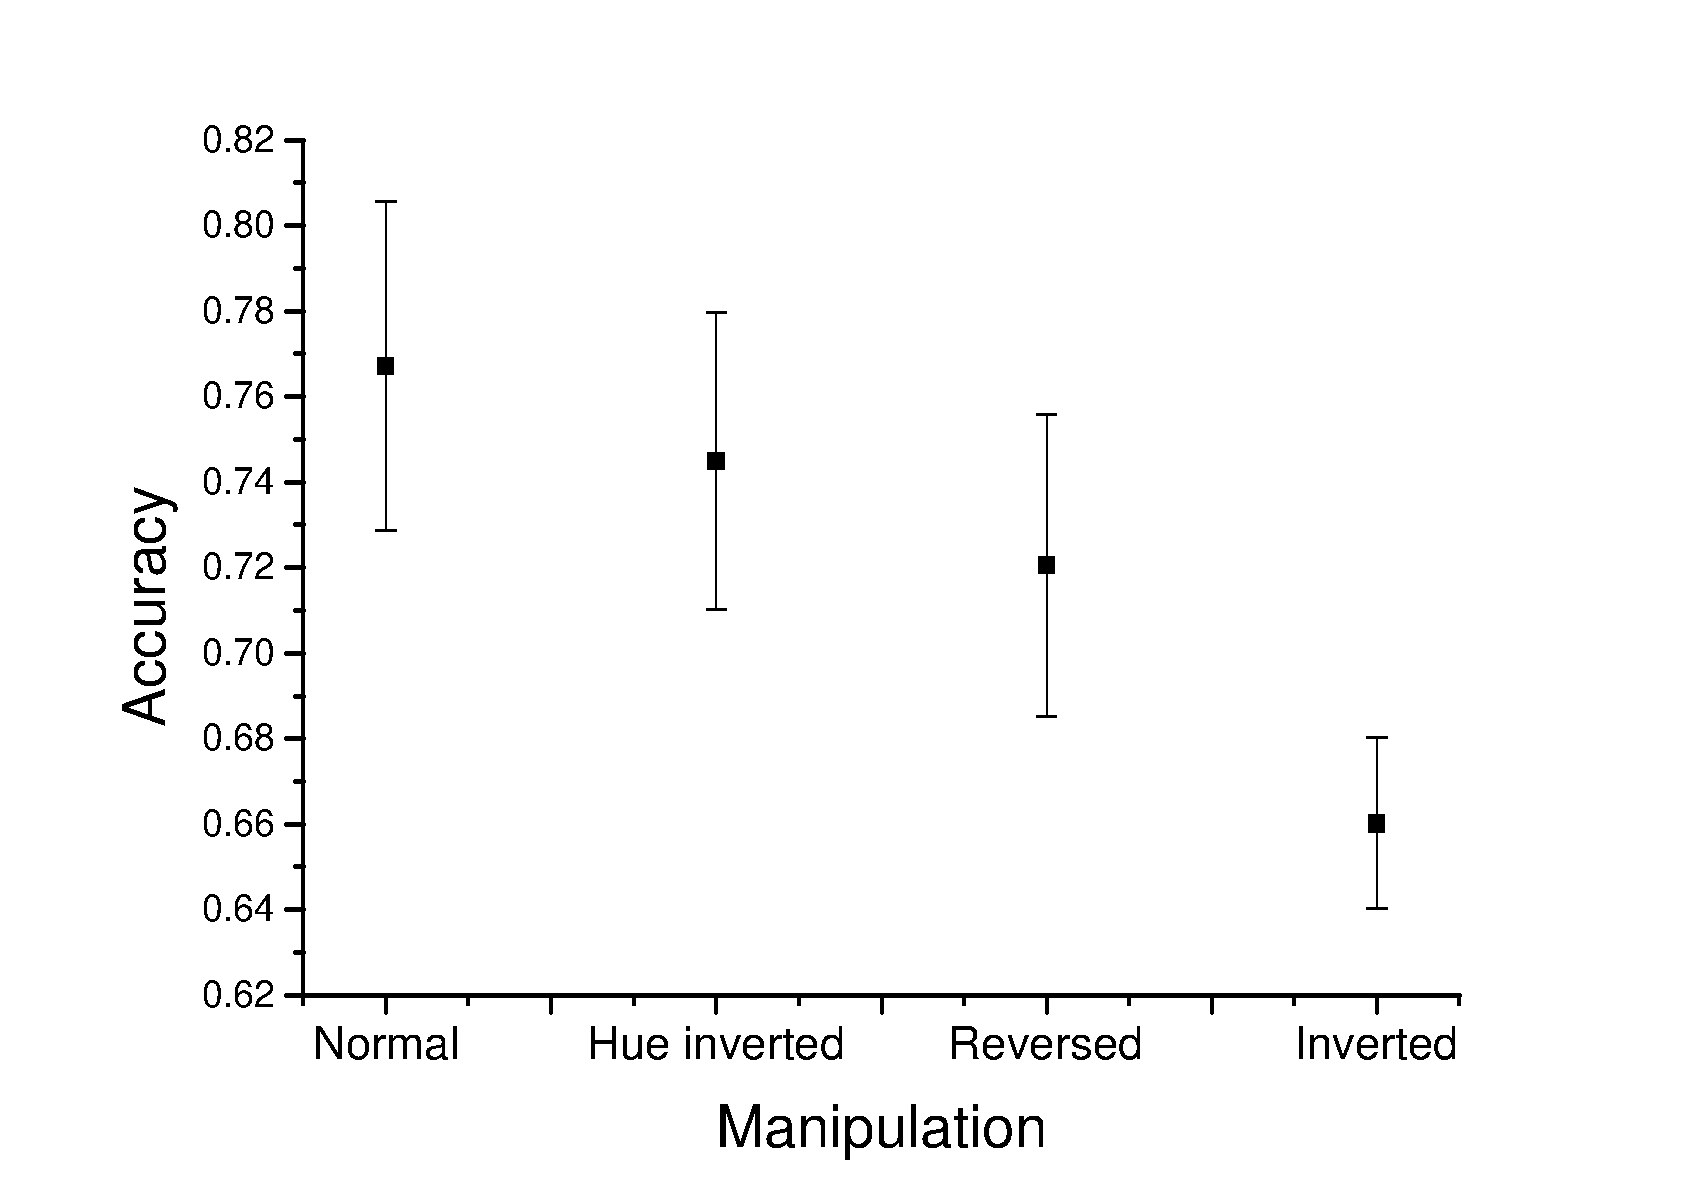
\includegraphics[width=\textwidth]{img/accuracyvsmanipulation.pdf}
    }
    \caption{\textbf{Experiment 3.} In a delayed-match-to-sample task, sample clips were altered by colour inversion, temporal inversion, and spatial inversion. This disrupted colour information, temporal order of features and spatial layout of features. Subjects needed to match a stored, altered percept with an incoming, unaltered clip. Decreases in accuracy showed which types of information were most important for matching: spatial configuration, followed by temporal order.}
    \label{fig:dummy}
  \end{figure}



\section{Are these representations specialised?}

Certain neural codes are specialised: they are adapted to representing specific stimulus classes. For example, (INSERT face cells).

The question of whether specialised codes exist for a certain stimulus group is very similar to that of whether an internal model of that group exists. An internal model forms specialised representations and, centrally, fills them in: it can fill in or interpolate absent details from given information. For example, on perceiving the bottom half of a face, one can often imagine the appearance of the upper half.

There is no question that we have a basic internal model of fire, because we can recognise it trivially and make simple judgements about its affordances and size. This model is also not perfect, because we cannot predict in detail what a fire is going to do (such a skill would require simulating a complex thermodynamic system, and immense processing power). We can, however, attempt to measure how good our model is.

Models are used to make judgements from stimuli. For example, expertise in face perception serves to guess at a conspecific's age, physical condition and current mental state. The better the model, the more accurate these judgements and the less information required to make them.

 We investigated the effect of reduced information on accuracy of a particular judgement of hearth fire clips. Given the importance of temporal order to fire perception, we asked participants to judge whether clips were being played forwards or backwards.

Whether played forwards or backwards, a clip contains the same sequence of frames and causes the same patterns of light to fall upon the retina. What differs is order. Being presented in reverse, these frames evoke opposite-direction motion percepts.

Our predictions were as follows. Consider a subject with a highly-developed model of flame. Normal clips would register well with this model, being perceived as real. Clips played in reverse, however, would evoke motion percepts which did not tally with those expected by the model, leading to a sensation of irreality.

Experiment 4 tested these predictions by showing a series of clips and requesting a "forwards-or-backwards" judgement after each clip. Clips varied in frame rate, with interframe delays ranging from 0.02 s (50 fps, the original frame rate) to 0.2 s (5 fps). Clips were also shown rotated by 0, 90, 180 or 270 degrees (Fig. REF). Rotation was varied across blocks, with 2 blocks per angle; frame rate was varied within blocks. Block order was randomised.

Mean accuracy was 90\% at full frame rate, but descended quickly to chance at 10 fps (interframe delay: 0.1 s). Subjects' internal models of fire were good at predicting reality when frames were close together, but found this task impossible with widely spaced frames.

This drop in accuracy means that the correlations encoded by the model are mostly short-range, concerning the relationships between frames close together in time. These representations of fire store local descriptions.

Skill at this task was already present, not acquired during the experiment. We plotted accuracy against progress through the task; performance did not significantly increase between the first and last quarters of the experiment. Forwards/backwards judgement therefore uses existing representations and processes, not new skills learned during the task.




\section{Are fire representations tuned to direction?}

Some representations are tuned to stimuli oriented in a particular direction.

In face recognition, the improved recognition of upright faces over inverted faces is termed the inversion effect. Although there is debate about its exact causes\cite{farah1995causes}, it is generally accepted as evidence of specialisation for face processing. The representation set which informs face recognition is better tuned to encoding upright faces, and thus it cannot encode inverted faces as effectively. This impairs recognition.

We checked for the presence of a similar effect in the task of fire discrimination, using two experiments. 

Firstly, Experiment 3 used the same delayed-match-to-sample paradigm as Experiment 1, with one factor only: in half the trials, the sample and candidate clips were both inverted. This tested the ability of the brain's representation set to store and evaluate codings of inverted fire clips. As shown in Fig (REF), there was no significant difference in recognition rates between upright and inverted clips. In fact, 50\% of subjects performed slightly better with inverted clips.

Secondly, we looked at recognition accuracies across the four rotation directions used in Experiment 4: upright, inverted, and rotated 90 degrees to the left and right. As shown in Fig (REF), there was once again no significant difference in accuracy across the rotation directions. 

In face recognition tasks, it is commonplace to find an accuracy drop of over 10\% with inverted faces\cite{freire2000face,yovel2005neural}. This large, decisive effect is not present with fire stimuli; inversion does not impair fire recognition as much as flame recognition.

This could be explained by fire representations which were direction-independent. With faces, the inversion effect seems to be due to mis-coding of configural information (faces which differ in feature configuration are recognised worse under inversion than faces which differ in feature identity\cite{freire2000face}); this information is highly vertically asymmetric, meaning that flipped configurations are badly encoded. With flames, the lack of an inversion effect indicates that the brain is as good at representing inverted fires as upright ones; its representations are symmetric. 

If the representations available to the fire comparison process were better at coding a specific direction of motion (as we could imagine, given that flaming gas usually moves upward), discrimination would suffer under rotation. However, as these encodings store enough information to allow differentiation of clips rotated by 180 degrees or by 90 degrees in either direction, we conclude that they not tuned specifically to motion in any direction.



\section{Conclusions}

Initial investigations of the cognitive processes which evaluate and perceive fire indicate that local correlations are represented well (NOTE direction exp), but also that longer clips provide more local detail which clouds discrimination (NOTE first 2 exps). This suggests that visually perceived fires are encoded as a bag of spatially and temporally local features.

Larger bags of features impair recognition. This could be because the local feature representations are used to generate a fixed-information global representation, which can only effectively store a certain amount of detail. Alternatively, it could be because more local representations are more costly to compare, and the matching process loses accuracy to minimise cost.



Its presence in the environment of the evolving 


We are thinking on a level between the neural and the cognitive, a level insufficiently detailed to model individual neurons but more specific than descriptions of qualia or percepts. Our main primitive is the concept of the \textit{neural representation}, a description of how a particular idea, metric or concept is coded by neural activity or architecture. It is illustrative to provide some examples.


A place cell, which fires when an animal occupies a particular area of its environment, is a representation of that particular location. Simiarly, a head direction cell represents orientation.

Visual information is encoded in many different representations as it passes from retina to cortex.




\bibliography{jovtemplate_latex}
\bibliographystyle{jovcite}

\end{document}

